% !TEX root = ../../../main.tex

\toggletrue{image}
\toggletrue{imagehover}
\chapterimage{add}
\chapterimagetitle{\uppercase{Add}}
\chapterimageurl{https://xkcd.com/1106/}
\chapterimagehover{\footnotesize 20 balloons float away while I'm busy permanently tying one to a tree to deal with it for good. Unfortunately, that one balloon was 'land a rocket on the moon in Kerbal Space Program.'}

\chapter{Volladdierer}
\label{ch:volladdierer}

Ein Halbaddierer reicht nicht aus, um zwei mehrstellige Dualzahlen zu addieren. Wir müssen in der Lage sein, drei Binärziffern zu addieren. Die Lernziele dieses Kapitels sind:\\

\lernziel{\autoref{ch:volladdierer}, \nameref{ch:volladdierer}}{
\begin{minipage}{\linewidth}
$\square$ \hspace{0.1cm} Sie erstellen ein Schaltnetz, das drei Binärziffern addieren kann.\\
$\square$ \hspace{0.1cm} Sie definieren, was ein Volladdierer ist.\\
$\square$ \hspace{0.1cm} Sie erklären die Notwendigkeit eines Volladdierers für die Addition mehrstelliger Dualzahlen.\\
$\square$ \hspace{0.1cm} Sie konstruieren einen Volladdierer unter der Verwendung von Halbaddierern.
\end{minipage}
}

\section{Konstruktion des Volladdierers}

Wir realisieren nun die Addition von \textbf{drei} Binär\textbf{ziffern} durch ein Schaltnetz. Dies geschieht bei der schriftlichen Addition von zwei mehrstelligen Dualzahlen in fast jeder Spalte, wie das folgende Beispiel zeigt.

\begin{figure}[htb]
\centering
\begin{equation*}
\begin{tikzpicture}[
    row 3/.style={font=\scriptsize},
    every node/.style={column sep=.5mm, row sep=1mm}]
    \matrix (m) [matrix of math nodes,
        nodes in empty cells,
        %nodes=draw
    ] 
    {
    		& 	& \textbf{1} & \textbf{0} & \textbf{1} & 1 & [5mm]	\text{1. Summand} \\
	+      & 	& \textbf{0} & \textbf{1} & \textbf{1} & 1 &      	\text{2. Summand} \\ 
		& 1 	& \textbf{1} & \textbf{1} & \textbf{1} &    &         	\text{Überträge} \\
        		& 1 	& 0 & 0 & 1 & 0 &      	 \text{Summe} \\                                                  
    };
    \draw[-,color=black, semithick] (m-3-1.south west) -- (m-3-6.south east);
\end{tikzpicture}
\end{equation*}
\end{figure}

Die Addition aber der zweiten Stelle setzt sich nun pro Stelle aus folgenden Komponenten zusammen:

\begin{itemize}
\item Die beiden Binärziffern ($x$ und $y$) der Summanden und die Binärziffer für den \textbf{ein}gehende Übertrag ($c_{\text{in}}$) aus der \textbf{vorherigen} Stelle.
\item Die Binärziffer $s$ für das Ergebnis der Addition (Summe).
\item Die Binärziffer für den \textbf{aus}gehenden Übertrag ($c_{\text{out}}$) für die \textbf{nächste} Stelle.
\end{itemize}

Wir können nun wie bei einem Halbaddierer vorgehen und das Schaltnetz für die Addition von drei Binärziffern erstellen.

\newpage

\subsection{Übungen}

Lösen Sie die Übungen in der vorgegebenen Reihenfolge.

\begin{exercise}\label{exercise-addition-drei-binarziffern-wahrheitstabelle}
Füllen Sie die Wahrheitstabelle (siehe \autoref{table-addition-drei-binarziffern}) aus. Die Wahrheitstabelle muss alle acht Kombinationen für die Addition von drei Binärziffern enthalten.

\begin{table}[htb]
\centering
\begin{tblr}{|Q[c, m, 2cm]|Q[c, m, 2cm]|Q[c, m, 2cm]||Q[c, m, 2cm]|Q[c, m, 2cm]|}
\hline
\SetCell[c=3]{c} Eingänge & & & \SetCell[c=2]{c} Ausgänge \\ \hline
$x$ & $y$ & $c_{\text{in}}$ & $s$ & $c_{\text{out}}$ \\ \hline[2pt]
0 & 0 & 0 & & \\ \hline
0 & 0 & 1 & & \\ \hline
0 & 1 & 0 & & \\ \hline
0 & 1 & 1 & & \\ \hline
1 & 0 & 0 & & \\ \hline
1 & 0 & 1 & & \\ \hline
1 & 1 & 0 & & \\ \hline
1 & 1 & 1 & & \\ \hline
\end{tblr}
\caption{Wahrheitstabelle für die Addition von drei Binärziffern. $x$ ist die Binärziffer des 1. Summanden und $y$ ist die Binärziffer des 2. Summanden. Der dritte Eingang ist der Übertrag aus der vorherigen Stelle (carry in, kurz $c_{\text{in}}$). Die Ausgänge bestehen aus der Summe $s$ und dem Übertrag für die nächste Stelle (carry out, kurz $c_{\text{out}}$).}
\label{table-addition-drei-binarziffern}
\end{table}
\end{exercise}

\begin{exercise}\label{exercise-addition-drei-binarziffern-dnf}
Erstellen Sie für die Wahrheitstabelle aus Übung \ref{exercise-addition-drei-binarziffern-wahrheitstabelle} (siehe \autoref{table-addition-drei-binarziffern}) eine boolesche Formel in \ac{DNF}. Sie müssen also für $s$ und $c_{\text{out}}$ \textbf{jeweils} eine boolesche Formel in \ac{DNF} erstellen. Falls Sie die \ac{KV}-Diagramme kennengelernt haben, dann erstellen Sie eine \textbf{vereinfachte boolesche Formel} in \ac{DNF}. Verwenden Sie dazu \textbf{zwei} \ac{KV}-Diagramme. Jedes Diagramm hat \textbf{drei} Eingänge.

\fillwithgrid{\stretch{1}}

\end{exercise}

\newpage

\begin{exercise}
Zeichen Sie zu den booleschen Formeln aus Übung \ref{exercise-addition-drei-binarziffern-dnf} das zugehörige Schaltnetz. Es handelt sich um \textbf{ein} Schaltnetz mit \textbf{drei} Eingängen und \textbf{zwei Ausgängen}.

\fillwithgrid{6in}

\end{exercise}

\begin{exercise}
Zeichnen Sie erneut das Schaltnetz für einen Volladdierer. Verwenden Sie diesmal jedoch nur \textbf{zwei Halbaddierer} und \textbf{ein \texttt{OR}-Gatter}.
\fillwithgrid{\stretch{1}}
\end{exercise}

\newpage

\section{Der Volladdierer}

Bei der Addition von zwei Dualzahlen muss ein Übertrag aus der vorhergehenden Stelle berücksichtigen werden. Wir nennen dies einen \textbf{eingehenden Übertrag} (engl. carry in, abgekürzt $c_{\text{in}}$). 

\begin{definition}[Volladdierer]
Ein Schaltnetz, das \textbf{drei} \textbf{einstellige} Dualzahlen (drei Binärziffern) addieren kann, wir als \textbf{Volladdierer} (engl. full adder, abgekürzt \acs{FA}) bezeichnet. Die dritte Binärziffer entspricht dabei dem eingehenden Übertrag aus der vorhergehenden Stelle. Die beiden Ausgänge stellen die Summe, sowie den ausgehenden Übertrag ($c_{\text{out}}$) dar.
\end{definition}

Es gibt mehrere Möglichkeiten, ein Schaltnetz für einen Volladdierer zu konstruieren. \autoref{full-adder-schaltnetz-1} zeigt eine Möglichkeit.

\begin{figure}[ht]
\centering
\begin{circuitikz}
\draw (0,0) node[xor port] (XOR1) {};
\draw (0, -1.5) node[and port] (AND1) {};
\draw (-5,0) node (x) {$x$};
\draw (x) to (-2,  0) node[circle, fill, inner sep=1pt] (xcross) {} |- (XOR1.in 1);
\draw (-2,  0) |- (AND1.in 1);
\draw (-5,-0.5) node (y) {$y$};
\draw (y) to (-2.5,  -0.5) node[circle, fill, inner sep=1pt] (ycross) {} |- (XOR1.in 2);
\draw (-2.5, -0.5) |- (AND1.in 2);
\draw (-5,-2.5) node (ci) {$c_{\text{in}}$};

\draw (3,0) node[xor port] (XOR2) {};
\draw (3, -1.5) node[and port] (AND2) {};
\draw (XOR1.out) to (0.5, 0) node[circle, fill, inner sep=1pt] (s1cross) {} |- (XOR2.in 1);
\draw (s1cross) |- (AND2.in 1);
\node[circle, fill, inner sep=1pt] (cicross2) at (AND2.in 2) {};
\draw (cicross2) {} |- (XOR2.in 2);
\draw (ci) to (1, -2.5) node (s1cross) {} |- (cicross2);

\draw (5, -2) node[or port] (OR1) {};
\draw (AND2.out) |- (OR1.in 1);
\draw (AND1.out) |- (OR1.in 2);
\draw (XOR2.out) to (6, 0) node[anchor=west] {$s$};
\draw (OR1.out) -+(6, -2) node[anchor=west] {$c_{\text{out}}$};
\end{circuitikz}
\caption{Das Schaltnetz stellt einen Volladdierer (\protect\say{White Box}) dar.}
\label{full-adder-schaltnetz-1}
\end{figure}

Unabhängig davon, wie wir das Schaltnetz für den Volladdierer (\ac{FA}) konstruieren, wir verwenden nun die Darstellung aus \autoref{figure-fa-block} für den Volladdierer.

\begin{figure}[htb]
\centering
\begin{circuitikz}[american]
	\ctikzset{multipoles/dipchip/width=2}
	\draw (0,0) node[dipchip, num pins=6, hide numbers, no topmark, draw only pins={1-4, 6}] (FA1) {\textbf{\acs{FA}}};
	\node [right] at (FA1.bpin 1) {$x$};
	\node [right] at (FA1.bpin 2) {$y$};
	\node [right] at (FA1.bpin 3) {$c_{\text{in}}$};

	\node [left] at (FA1.bpin 6) {$s$};
	\node [left] at (FA1.bpin 4) {$c_{\text{out}}$};
\end{circuitikz}
\caption{Ein Volladdierer (\protect\say{Black Box}) mit drei Eingängen und zwei Ausgängen.}
\label{figure-fa-block}
\end{figure}

\subsection{Übungen}

\begin{exercise}
Ein Halbaddierer kann die Addition von zwei \textbf{mehrstelligen} Dualzahlen die Addition in der \textbf{ersten} Spalte durchführen. Für alle weiteren Spalten wird jeweils ein Volladdierer benötigt. Notieren Sie jeweils die Anzahl der Halb- und Volladdierer für die folgenden Additionen:

\begin{multicols}{3}
\begin{itemize}
\item zwei \num{3}-Bit-Dualzahlen
\item zwei \num{8}-Bit-Dualzahlen
\item zwei \num{10}-Bit-Dualzahlen
\end{itemize}
\end{multicols}
\end{exercise}

\begin{exercise}
Stellen Sie den Ablauf der Addition zweier beliebiger \num{3}-Bit-Dualzahlen grafisch dar. Die Bits der beiden Summanden werden mit $x_i$ und $y_i$ bezeichnet. Die Bits der Summe werden mit $s_i$ abgekürzt. Stellen Sie auch eingehende und ausgehende Überträge dar. In die Rechtecke ist entweder \ac{HA} für Halbaddierer oder \ac{FA} für Volladdierer einzutragen.

\begin{figure}[H]
\centering
\begin{minipage}{0.2\textwidth}
\centering
\begin{adjustbox}{width=\textwidth}
\begin{tblr}{ccccc}
   	& & $x_2$ & $x_1$ & $x_0$ \\
+ 	& & $y_2$ & $y_1$ & $y_0$ \\
    	& {\scriptsize $c_2$}  & {\scriptsize $c_1$} & {\scriptsize $c_0$} & \\
\hline
	& $s_3$ & $s_2$ & $s_1$ & $s_0$ \\
\end{tblr}
\end{adjustbox}
\end{minipage}
\hfill
\begin{minipage}{0.7\textwidth}
\centering
\begin{adjustbox}{width=\textwidth}
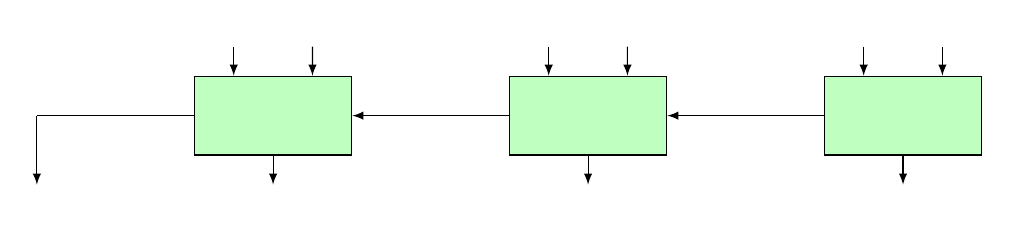
\begin{tikzpicture}

\node[rectangle, draw, fill=green!25, minimum width=2cm, minimum height=1cm] (r0) at (0, 0) {};
\node (x0) at (0.5, 1) {};
\node (y0) at (-0.5, 1) {};
\node (s0) at (0, -1) {};
\draw[-latex] (x0) -- ([xshift=+0.5cm]r0.north);
\draw[-latex] (y0) -- ([xshift=-0.5cm]r0.north);
\draw[-latex] (r0.south) -- (s0);

\node[rectangle, draw, fill=green!25, minimum width=2cm, minimum height=1cm] (r1) at (-4, 0) {};
\node (x1) at (-3.5, 1) {};
\node (y1) at (-4.5, 1) {};
\node (s1) at (-4, -1) {};
\draw[-latex] (x1) -- ([xshift=+0.5cm]r1.north);
\draw[-latex] (y1) -- ([xshift=-0.5cm]r1.north);
\draw[-latex] (r1.south) -- (s1);

\draw[-latex] (r0.west) -- node[above] {} (r1.east);

\node[rectangle, draw, fill=green!25, minimum width=2cm, minimum height=1cm] (r2) at (-8, 0) {};
\node (x2) at (-7.5, 1) {};
\node (y2) at (-8.5, 1) {};
\node (s2) at (-8, -1) {};
\draw[-latex] (x2) -- ([xshift=+0.5cm]r2.north);
\draw[-latex] (y2) -- ([xshift=-0.5cm]r2.north);
\draw[-latex] (r2.south) -- (s2);

\draw[-latex] (r1.west) -- node[above] {} (r2.east);

\node (tmp) at (-11, 0) {};
\node (s3) at (-11, -1) {};

\draw (r2.west) -- node[above] {} (tmp.center);
\draw[-latex] (tmp.center) -- (s3);

\end{tikzpicture}
\end{adjustbox}

\end{minipage}
\end{figure}
\end{exercise}
